\documentclass{beamer}
\usetheme{Singapore}

\usepackage{amsmath,amssymb,latexsym}
\usepackage{graphicx}
\usepackage{fancyvrb}
\usepackage{hyperref}

\newcommand{\bi}{\begin{itemize}}
\newcommand{\ii}{\item}
\newcommand{\ei}{\end{itemize}}
\newcommand{\Show}[1]{\psshadowbox{#1}}

\newcommand{\set}[1]{\ensuremath{\left\{ #1 \right\}}}
\newcommand{\nats}{\ensuremath{\mathbb{N}}}
\newcommand{\nni}{\ensuremath{\mathbb{N}^0}}
\newcommand{\ints}{\ensuremath{\mathbb{Z}}}
\newcommand{\power}{\ensuremath{\mathcal{P}}}
\renewcommand{\neg}{\sim}
\newcommand{\xor}{\oplus}
\newcommand{\then}{\ensuremath{\Rightarrow}}


\newcommand{\grf}[2]{\centerline{\includegraphics[width=#1\textwidth]{#2}}}
\newcommand{\tw}{\textwidth}
\newcommand{\bc}{\begin{columns}}
\newcommand{\ec}{\end{columns}}
\newcommand{\cc}[1]{\column{#1\textwidth}}

\newcommand{\bfr}[1]{\begin{frame}[fragile]\frametitle{{ #1 }}}
\newcommand{\efr}{\end{frame}}

\newcommand{\cola}[1]{\begin{columns}\begin{column}{#1\textwidth}}
\newcommand{\colb}[1]{\end{column}\begin{column}{#1\textwidth}}
\newcommand{\colc}{\end{column}\end{columns}}

\title{Book of Proof: Fundamentals}

\RecustomVerbatimEnvironment{Verbatim}{Verbatim}{frame=single}

\begin{document}
\begin{frame}
\maketitle

\end{frame}

\bfr{Sets: A mathematical structure}



\begin{align*}
&  \{1,2,3\} \\
&  \set{a,b,c,d} \\
&  \set{cat, dog, pig}\\
&  \set{2,4,6,8,...}\\
  \emptyset &= \{\}\\
  \emptyset &\not= \{\emptyset\}\\
\end{align*}

Note: \set{1,2,3} is not the same as \ensuremath{1,2,3} or \ensuremath{(1,2,3)} or {\em etc.}

\end{frame}

\bfr{Sets have no order or duplicates}
\begin{align*}
  \{1,2,3\}
&= \{2,3,1\}\\
&= \{2,1,3\}\\
  &=  \{1,1,2,2,3,3\} \\
&= \{2,3,3,2,1,1,1,1,2,3,2,2,2,3,1\}\\
\end{align*}


\end{frame}

\bfr{Some important sets}
The integers, the natural numbers, the nonnegative integers
\begin{align*}
  \mathbb{Z} &= \{...,-3,-2,-1,0,1,2,3,4,...\} \\
  \mathbb{N} &= \{1,2,3,4,...\}  \\
  \mathbb{N}^0 &= \{0,1,2,3,4,...\}  \\
\end{align*}

We won't have much use for the real numbers, $\mathbb{R}$.
\end{frame}

\bfr{The size of a finite set}
\begin{align*}
3 &=  |\{a,b,c\}| \\
5 &=  |\{a,b,c,d,e\}| \\
 &=  |\{a,b,c,d,e,a,d,b\}| \\
0 &=  |\emptyset| \\
1 &=  |\{\emptyset\}| \\  
1 &=  |\{\{\emptyset\}\}| \\  
\end{align*}

\end{frame}

\bfr{Membership and subsets}
\begin{align*}
  3 &\in \set{1,2,3,4,5}\\
  3 &\not\in \set{2,4,6,8}\\
  cat &\in \set{cat, dog, pig}\\
  3 &\in \nni\\
  \pi &\not\in \ints\\
  \\
  \set{2,5,8} &\subseteq \set{1,2,3,4,5,6,7,8,9,10}\\
  \set{2,5,8} &\not\subseteq \set{1,2,3,4,5,6,7}\\
  \set{3} &\subseteq \set{1,2,3,4,5}\\
  \set{3} &\not\subseteq \set{2,4,6,8}\\
  \nni &\subseteq \ints \\
  \mathbb{R} &\not\subseteq \nats
  \end{align*}

\end{frame}
\bfr{Set builder notation}
\begin{align*}
  \set{n : \mbox{$n$ is odd and $4\leq n \leq 16$}}
  &= \set{5,7,9,11,13,15}\\
  \set{2n+5 : n\in\set{3,6,7}} &= \set{11,17,19}\\
  \set{2n: n\in\nni} &= \set{0,2,4,6,8,...}\\
  \set{n\in\nats : n < 5} &= \set{1,2,3,4}\\
  \set{3n: n\in\nats \mbox{ and } n < 5} &= \set{3,6,9,12}\\
\end{align*}

\end{frame}

\bfr{Ordered pairs, triples, $n$-tuples}
\begin{align*}
  (2,4) &\not= (4,2)\\
  (2,2) &\not= (2)\\
  (1,2,3) &\not=(3,2,1)\\
  (1,1,2) &\not=(1,2)\\
  (5,3,2,1,6) &\not= (1,2,3,5,6)\\
\end{align*}
\end{frame}

\bfr{Cartesian product}
  
\begin{align*}
A \times B &= \set{(x,y) : x\in A \mbox{ and } y \in B}\\
\set{a,b}\times\set{1,2,3} &= \set{
  (a,1), (a,2), (a,3), (b,1), (b,2), (b,3)}\\
\end{align*}

If $A$ and $B$ are finite sets, then $|A\times B| = |A|\cdot|B|$.
\end{frame}

\bfr{Higher order Cartesian products}
\begin{align*}
  A\times B\times C &= \set{(a,b,c) : a\in A,b\in B, c\in C}\\
  A^n &= A\times A\times A \times... \times A\\
   &= \set{(x_1, x_2, x_3, ..., x_n) : x_1,x_2,x_3,...,x_n\in A}\\
\end{align*}
\end{frame}

\bfr{Power set: the set of all subsets}

\begin{align*}
  \power(\set{a,b,c}) &= \set{\emptyset,\set{a},\set{b},\set{c},
    \set{a,b},\set{a,c},\set{b,c},\set{a,b,c}}
\end{align*}

How many subsets are there?
\end{frame}


\bfr{If $|A| = n$ then $|\power(A)| = 2^n$}

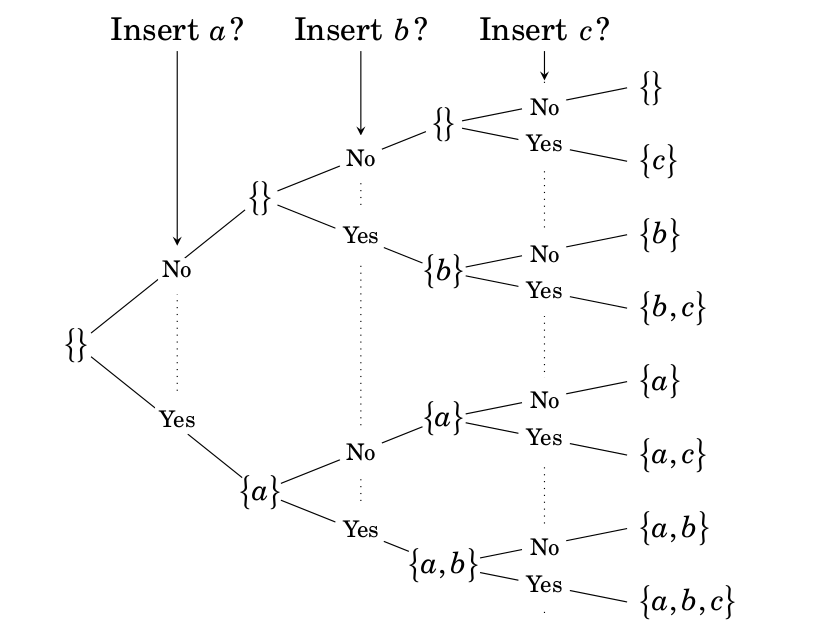
\includegraphics[width=.8\textwidth]{powersettree.png}

\end{frame}


\bfr{Union, Intersection, Difference}
\begin{align*}
  A\cup B &= \set{x : x\in A \mbox{ or } x \in B}\\
  A\cap B &= \set{x : x\in A \mbox{ and } x \in B}\\
  A - B &= \set{x : x\in A \mbox{ and } x \not\in B}\\
  \\
  A &= \set{1,2,3,4,5}\\
  B &= \set{4,5,6,7,8}\\
  A \cup B &= \set{1,2,3,4,5,6,7,8}\\
  A \cap B &= \set{4,5}\\
  A - B &= \set{1,2,3}\\
  \end{align*}

\end{frame}

\bfr{Complement}
\begin{align*}
  \overline{A} &= \set{x : x\not\in A}\\
  \\
  \overline{\set{2,4,6,8,...}} &= \set{1,3,5,7,...}\\
\end{align*}

Usually relative to some implied {\bf universal set} or {\bf universe},
in this case, \nats.

\end{frame}

\bfr{Indexed Sets}
\begin{align*}
  \bigcup_{i=1}^n A_i &= A_1 \cup A_2 \cup A_3 \cup ... \cup A_n\\
  \bigcap_{i=1}^n A_i &= A_1 \cap A_2 \cap A_3 \cap ... \cap A_n\\
\end{align*}
\end{frame}

\bfr{Indexed Sets}
\begin{align*}
  A_i &= \set{ni : n\in\nats}\\
  A_1 &= \set{1,2,3,4,...}\\
  A_2 &= \set{2,4,6,8,...}\\
  A_3 &= \set{3,6,9,12,...}\\
  A_4 &= \set{4,8,12,16,...}\\
      &...\\
  \\
  \bigcup_{i=2}^4 A_i &= \set{2,3,4,6,8,9,10,12,14,15,...}\\
  \bigcap_{i=2}^4 A_i &= \set{12,24,36,48,72,...}\\
\end{align*}
\end{frame}

\bfr{Logic}
\begin{enumerate}
\item Circle $X$ has radius equal to 3.
\item If any circle has radius $r$, then its area is $\pi r^2$.
  
  \hrulefill
\item Circle $X$ has area $9\pi$.
\end{enumerate}

\end{frame}

\bfr{Statements}

\begin{tabular}{|l|l|}\hline
  NOT Statements: & Statements \\\hline\hline
  Add 5 to both sides. &
  \parbox{2in}{Adding 5 to both sides of\\ $x-5=37$ gives $x=42$.}\\\hline
  $\mathbb{Z}$ & $42\in\mathbb{Z}$ \\\hline
  42 & 42 is not a number. \\\hline
  What is the solution of $2x=84$? & The solution of $2x=84$ is 42.\\\hline
\end{tabular}

\vfill

We use the letters $P$, $Q$, $R$ and $S$ to stand for statements.

\end{frame}

\bfr{Examples}
\begin{tabular}{lll}
  $P$&:& The function $f(x)=x^2$ is continuous. \\
  $P(x)$&:& If an integer $x$ is a multiple of 6, then $x$ is even.\\
  $Q(x)$&:& The integer $x$ is even.\\
\end{tabular}
\vfill

A sentence whose truth value depends on the value of variables
is called an {\bf open sentence}.
\end{frame}

\bfr{And, Or, Not}
\begin{tabular}{lll}
  $P$&: & The number 4 is even.\\
  $Q$&: & The number 7 is even.\\
  $P\wedge Q$&: & The number 4 is even {\bf and} the number 7 is even.\\
  $P\vee Q$&:& The number 4 is even {\bf or} the number 7 is even.\\
  $\neg P$&:& The number 4 is {\bf not} even.\\
  $\neg Q$&:& The number 7 is {\bf not} even.\\
\end{tabular}
\end{frame}

\bfr{Truth Tables}
\begin{tabular}{|c|c|c|}\hline
  $P$ & $Q$ & $P\land Q$ \\\hline
  $T$ & $T$ & $T$ \\\hline
  $T$ & $F$ & $F$ \\\hline
  $F$ & $T$ & $F$ \\\hline
  $F$ & $F$ & $F$ \\\hline
\end{tabular}\hfill
\begin{tabular}{|c|c|c|}\hline
  $P$ & $Q$ & $P\lor Q$ \\\hline
  $T$ & $T$ & $T$ \\\hline
  $T$ & $F$ & $T$ \\\hline
  $F$ & $T$ & $T$ \\\hline
  $F$ & $F$ & $F$ \\\hline
\end{tabular}

\vfill

\begin{tabular}{|c|c|}\hline
  $P$ & $\neg P$ \\\hline
  $T$ & $F$ \\\hline
  $F$ & $T$ \\\hline
\end{tabular}\hfill
\begin{tabular}{|c|c|c|}\hline
  $P$ & $Q$ & $P\xor Q$ \\\hline
  $T$ & $T$ & $F$ \\\hline
  $T$ & $F$ & $T$ \\\hline
  $F$ & $T$ & $T$ \\\hline
  $F$ & $F$ & $F$ \\\hline
\end{tabular}\hfill
\end{frame}

\bfr{Conditional Statements}
\begin{tabular}{rcl}
  $R(a)$ &:& {\bf If} the integer $a$ is multiple of 6,
  {\bf then} $a$ is divisible by 2.\\
  $P(a)$ &:& The integer $a$ is multiple of 6.\\
  $Q(a)$ &:& $a$ is divisible by 2.\\
  $R(a)$ &:& If $P$, then $Q$.\\
  $R(a)$ &:& $P \then Q$\\
\end{tabular}
\vfill

\begin{tabular}{|c|c|c|}\hline
  $P$ & $Q$ & $P\then Q$ \\\hline
  $T$ & $T$ & $T$ \\\hline
  $T$ & $F$ & $F$ \\\hline
  $F$ & $T$ & $T$ \\\hline
  $F$ & $F$ & $T$ \\\hline
\end{tabular}\hfill

\end{frame}


\bfr{Indexed Sets}
\[
\left.
\begin{array}{l}
  \mbox{If $P$ then $Q$.} \\
  \mbox{$P$ only if $Q$.}\\
  \mbox{$Q$, if $P$.}\\
  \mbox{$Q$ whenever $P$.}\\
  \mbox{$Q$, provided that $P$.}\\
  \mbox{Whenever $P$, then also $Q$.}\\
  \mbox{$P$ is sufficient for $Q$.}\\
  \mbox{$Q$ is necessary for $P$.}\\
\end{array}
\right\} P\then Q  
\]
\end{frame}


\bfr{Biconditional or Equivalence Statements}
\[
\left.
\begin{array}{l}
  \mbox{$P$ if and only if $Q$.} \\
  \mbox{$P$ iff $Q$.} \\
  \mbox{$P$ is necessary and sufficient for $Q$.}\\
  \mbox{If $P$, then $Q$, and conversely.}\\
\mbox{$P$ is logically equivalent to $Q$.}\\
(P\then Q)\land(Q\then P)\\
\end{array}
\right\} P\iff Q  
\]

\vfill

\begin{center}
\begin{tabular}{|c|c|c|}\hline
  $P$ & $Q$ & $P\iff Q$ \\\hline
  $T$ & $T$ & $T$ \\\hline
  $T$ & $F$ & $F$ \\\hline
  $F$ & $T$ & $F$ \\\hline
  $F$ & $F$ & $T$ \\\hline
\end{tabular}\hfill
\end{center}
\end{frame}


\bfr{Truth Tables for Complex Statements}
\newcommand{\row}[6]{$#1$&$#2$&$#3$&$#4$&$#5$&$#6$\\\hline}
\begin{tabular}{|c|c||c|c|c|c|}\hline
  $P$ & $Q$ & $(P\lor Q)$ & $(P\land Q)$ &  $\neg(P\land Q)$ &
  $(P\lor Q)\lor  \neg(P\land Q)$ \\\hline\hline
  \row TTTTFF
  \row TFTFTT
  \row FTTFTT
  \row FFFFTF
  \end{tabular}
  
\end{frame}

\bfr{Quantifiers}

Universal quantifier
\begin{itemize}
\item
For every $n\in\ints$, $2n$ is even.
\item
$\forall n \in \ints, 2n \mbox{ is even.}$
\item
  $\forall n \in \ints, E(2n)$
\end{itemize}
Existential quantifier
\begin{itemize}
\item
There exists a subset $X$ of \nats\ for which $|X| = 5$.
\item
$\exists X, (X\subseteq \nats)\land(|X|=5)$
\item
$\exists X \subseteq \nats, |X|=5$
\item
$\exists X\in\power( \nats), |X|=5$
\end{itemize}
\end{frame}

\bfr{Negating statements}
\begin{align*}
  \neg(P\then Q) &\iff P \land (\neg Q)\\
  \neg(P\land Q) &\iff (\neg P)\lor (\neg Q)\\
  \neg(P\lor Q) &\iff (\neg P)\land (\neg Q)\\
  \neg(\forall x\in S, P(x)) &\iff \exists x\in S, \neg P(x)\\
  \neg(\exists x\in S, P(x)) &\iff \forall x\in S, \neg P(x)\\
\end{align*}
\end{frame}

\bfr{Negating Statements, Example}
\begin{tabular}{rcl}
  $R$  &:& The square of every real number is non-negative.\\
  $R$  &:& $\forall x\in\mathbb{R}, x^2\geq 0$\\
  $\neg R$ &:&$\neg(\forall x\in\mathbb{R}, x^2\geq 0)$\\
  $\neg R$ &:&$\exists x\in\mathbb{R}, \neg(x^2\geq 0)$\\
  $\neg R$ &:&$\exists x\in\mathbb{R}, x^2 < 0$\\
  $\neg R$ &:& There exists a real number whose square is negative.\\
\end{tabular}

\end{frame}

\bfr{Negating Statements, Example}

$R$ : \\
{For every real number $x$
    there is a real number $y$ 
    for  which $y^3 = x$.}  

\begin{align*}
  R &= \forall x\in\mathbb{R}, \exists y\in\mathbb{R}, y^3 = x\\
  \neg R
  &= \neg(\forall x\in\mathbb{R}, \exists y\in\mathbb{R}, y^3 =  x)\\
  &= \exists x\in\mathbb{R}, \neg(\exists y\in\mathbb{R}, y^3 =  x)\\
  &= \exists x\in\mathbb{R}, \forall y\in\mathbb{R}, \neg(y^3 =  x)\\
  &= \exists x\in\mathbb{R}, \forall y\in\mathbb{R}, y^3 \neq  x\\
\end{align*}

$\neg R$ : \\
There is a real number $x$ for which $y^3 \neq x$ for all real
numbers $y$.

\end{frame}


\bfr{Tuples or Lists or Strings}
\begin{align*}
  (a,b,c,d,e) &\neq (b,a,c,d,e)\\
  (a,b,c,d,e)  &\neq (a,a,b,c,d,e)\\\\
  SOS &= (S,O,S)\\
\end{align*}
\end{frame}

\bfr{Counting Tuples: Multiplication Principle}
How many different lists of length 3 are there, where\\
the first entry must be an element of \set{a,b,c},\\
the second entry must be an element of \set{5,7},\\
and the third entry must be an element of \set{a,x}?


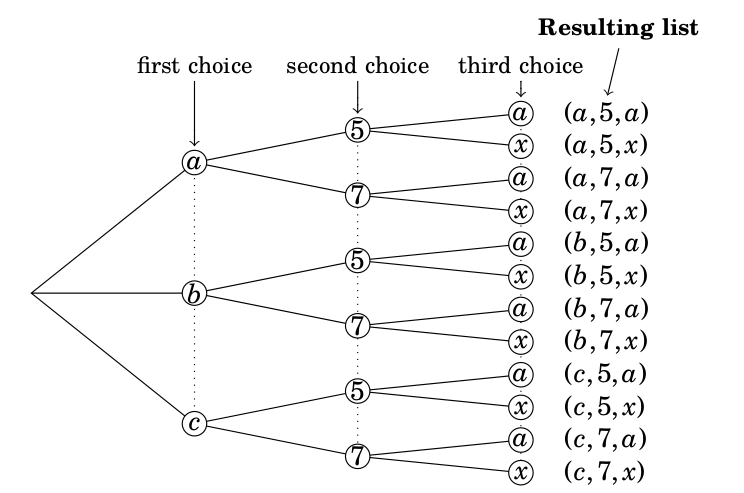
\includegraphics[width=0.8\textwidth]{listchoicetree.png}

\end{frame}

\bfr{Some notation: falling factorial powers}
\begin{align*}
  7^5 &= 7\cdot 7\cdot 7\cdot 7\cdot 7\\
  7^{\underline{5}} &= 7\cdot 6 \cdot 5\cdot 4\cdot 3\\
  7! &= 7\cdot 6 \cdot 5\cdot 4\cdot 3\cdot 2\cdot 1\\
  &= 7^{\underline{7}}\\
\end{align*}
\end{frame}

\bfr{Lists with repetitions}
How many lists of length 4 with selections from \set{A,B,C,D,E,F,G},
where repetition is allowed?
\pause


\centerline{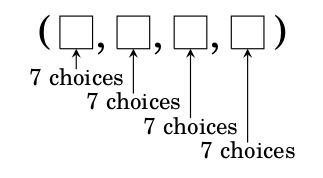
\includegraphics[scale=0.5]{choiceswithreps.png}}
\pause

\[ 7 \cdot 7 \cdot 7 \cdot 7 = 7^4\]
\end{frame}

\bfr{Lists without repetitions}
How many lists of length 4 with selections from \set{A,B,C,D,E,F,G},
where repetition is not allowed?
\pause

\centerline{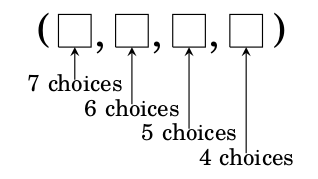
\includegraphics[scale=0.5]{choiceswithoutreps.png}}
\pause

\[ 7\cdot 6 \cdot 5\cdot 4 = 7^{\underline{4}}\]



\end{frame}

\bfr{More complex lists}
How many lists of length 4 with selections from \set{A,B,C,D,E,F,G},
without repetitions, and the symbol $E$ must appear somewhere in the
list?
\pause

\centerline{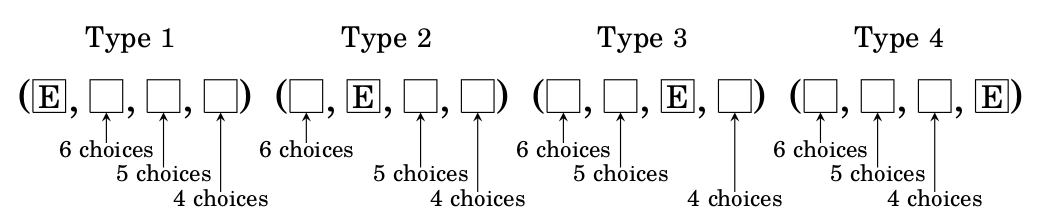
\includegraphics[width=\textwidth]{choiceswithe.png}}
\pause

\[ 4\cdot 6 \cdot 5\cdot 4 = 4\cdot 6^{\underline{3}} \]

\end{frame}

\bfr{More complex lists}
How many lists of length 4 with selections from \set{A,B,C,D,E,F,G},
repetition is allowed, and the list must contain an $E$?
\pause
\begin{itemize}
\item
There are $7^4$ lists where repetition is allowed.
\pause
\item
There are $6^4$ lists that do not contain $E$.
\pause
\end{itemize}
\[
7^4 - 6^4
\]

\end{frame}


\bfr{More about falling factorial powers}
\begin{align*}
  7^{\underline{3}} &= 7\cdot 6 \cdot 5\\
  7! &= 7\cdot 6 \cdot 5\cdot 4\cdot 3\cdot 2\cdot 1\\
  7^{\underline{3}} &=
  \frac{7\cdot 6 \cdot 5\cdot 4\cdot 3\cdot 2 \cdot 1}
       {4\cdot 3\cdot 2\cdot 1}\\
       &= \frac{7!}{4!}\\
       &= \frac{7!}{(7-3)!}\\
  n^{\underline{k}} &= \frac{n!}{(n-k)!}\\
  n! &= n^{\underline{n}}\\
\end{align*}
\end{frame}

\bfr{Permutations}
How many lists with repetitions of length $k$
can be made from $n$ symbols? \hfill $AAAA, BBBB, BABA, EBAB, CABC, ...$
\pause
\begin{align*}
  n^{{k}} 
\end{align*}
\pause
How many lists without repetitions of length $k$
can be made from $n$ symbols? \hfill $ABCD, DCBA, BCDE, EBAC, CABE, ...$
\pause
\begin{align*}
  n^{\underline{k}}
\end{align*}
\pause
\[
\frac{n!}{(n-k)!}
\]

\end{frame}

\bfr{Counting subsets}
How many subsets of size $k$ can be made by selecting elements from a
set of size $n$?

\pause

The number of lists without repetitions?
\pause
\[
n^{\underline{k}}
\]
But these contain set-equivalent pairs, such as $abc$ and $cba$.

\end{frame}

\bfr{Eliminating the duplicates}
\[
  \binom{5}{3}3! = 5^{\underline{3}} 
\]

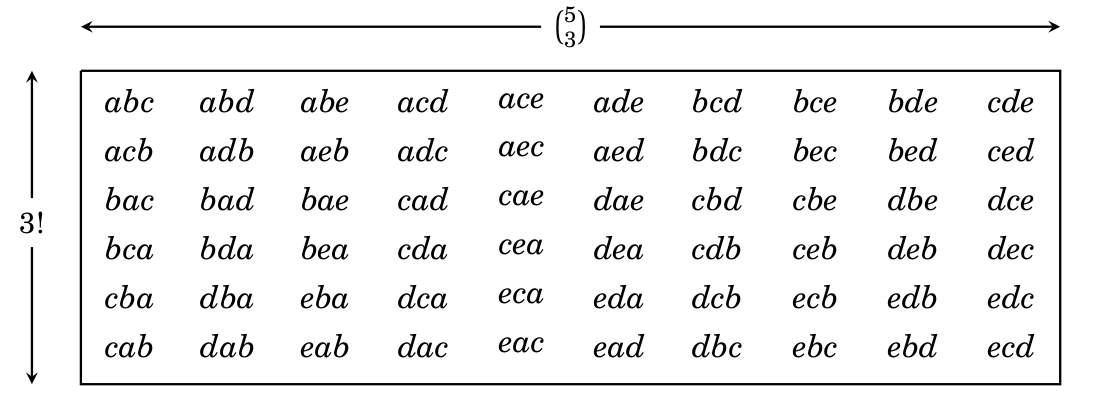
\includegraphics[width=\textwidth]{permstocombs.png}
\pause

\[
\binom{5}{3}
  = \frac{5!}{3!(5-3)!}
  = \frac{5^{\underline{3}}}{3!}
   = \frac{5^{\underline{3}}}{3^{\underline{3}}}
\]

\end{frame}
\bfr{Counting subsets}
How many subsets of size $k$ can be made by selecting elements from a
set of size $n$?
\pause

\[
\binom{n}{k}
  = \frac{n!}{k!(n-k)!}
  = \frac{n^{\underline{k}}}{k!}
   = \frac{n^{\underline{k}}}{k^{\underline{k}}}
\]
\end{frame}

\bfr{Easy to prove theorem?}
\[
\binom{n}{k} = \binom{n}{n-k}
\]
\end{frame}

\bfr{Using set theory in counting}
\[
|A\cup B| = |A| + |B| - |A\cap B|
\]

How many 3-card hands are there for which all 3 cards are red, or all
three cards are face cards?

$A =$ 3-card hands, all red cards\hfill  $B =$ 3-card hands, all face cards

\begin{align*}
  |A| &= \binom{13}{3}\\
  |B| &= \binom{12}{3}\\
  |A\cap B| &= \binom{6}{3}\\
  |A\cup B| &= |A| + |B| - |A\cap B|
  = \binom{13}{3} + \binom{12}{3} - \binom{6}{3}
\end{align*}



\end{frame}

\end{document}
